% UTF-8

% single-chapter commands
\documentclass[../main/thesis.tex]{subfiles}
\onlyinsubfile{\setcounter{chapter}{6}}  % single-chapter command
\begin{document}


\chapter{Schlussfolgerungen und Ausblick}
\label{ch:conclusion}

\section{Praktische Anwendbarkeit}

Es konnte durch die Implementierung in Software gezeigt werden, dass die Erkennung paralleler Linienzüge auf der Basis eines geometrischen Vergleichs möglichst kurzer Fragmente prinzipiell funktioniert.
Mit hierfür entwickelten Algorithmen können auch viele schwierige Situationen des in Abschnitt~\ref{ch:case-comparison} ausgewählten Spezialfalls der „baulich getrennten Richtungsfahrbahnen im Straßenraum“ zufriedenstellend gelöst werden.

Im Vergleich zu den in Abschnitt~\ref{ch:existing-approaches} diskutierten Ansätzen sind keine offensichtlichen grundsätzlichen Nachteile der mit der vorliegenden Arbeit entwickelten Methode zu erkennen.
Bei der Anwendung auf komplexe Straßennetze zeigt sich jedoch, dass erhebliche Probleme im Kreuzungsbereich, wie sie bereits von anderen Ansätzen ähnlich berichtet wurden, auch bei den in dieser Arbeit vorgestellten Algorithmen auftreten (siehe Abschnitt~\ref{ch:result-junctions}).
Aus Zeitgründen konnten praxistaugliche Lösungen hierfür nicht mehr als Teil dieser Arbeit entwickelt werden.

Die praktische Anwendbarkeit der entwickelten Algorithmen ist deshalb beschränkt.
Abschnitt~\ref{ch:improvements} diskutiert Wege, um das mögliche Einsatzgebiet zu erweitern.

Ferner darf hinterfragt werden, ob die Vorgabe der Aufgabenstellung hinsichtlich der Praxistauglichkeit der zu entwickelnden Algorithmen in Anbetracht der zeitlichen Begrenzung angemessen war.
Zwar ist Praxistauglichkeit immer anzustreben; wie schnell sie sich tatsächlich erreichen lässt, kann jedoch von Umständen abhängen, die nicht vollumfänglich vorherzusehen sind.
Auch ist zu bedenken, dass \citeauthor{LM96} den Umfang ihrer Arbeit, welcher eine vergleichbare Problemstellung zugrunde liegt, auf etwa sieben Personenmonate schätzen (siehe Abschnitt~\ref{ch:skeleton}). \cf{LM96}
Angesichts der im Rahmen der vorliegenden Arbeit aufgetretenen technischen Probleme ist nicht zu erwarten, dass der Aufwand für die Entwicklung einer praxistauglichen Lösung wesentlich geringer wäre.



\section{Möglichkeiten zur Weiterentwicklung}
\label{ch:improvements}



\subsection{Berücksichtigung unterschiedlicher Straßentypen}
% vgl. 6.1

Wie schon in Abschnitt~\ref{ch:result-trivial} erläutert, unterscheiden sich die optimalen Werte für die in Abschnitt~\ref{ch:analyse-algorithm} zur Definition von \textproc{Parallel} benutzten baulichen Kriterien für Abstand und Winkel der Richtungsfahrbahnen je nach Straßentyp.
Es wäre deshalb sinnvoll, diese Kriterien je nach Klassifikation der Straßen in der \osm-Datenbank entsprechend zu variieren.
Die Fehlerrate in der Erkennung würde dadurch sinken.

Diese geringfügige Verbesserung konnte lediglich aus Zeitgründen nicht mehr als Teil dieser Arbeit umgesetzt werden.



\subsection{Statistische Auswertung}
\label{ch:improvements-stats}
% vgl. 6.2

Attribute werden bei der \textproc{Analyse} nach Abschnitt~\ref{ch:analyse-algorithm} nur als hartes Ausschlusskriterium verwendet.
Abschnitt~\ref{ch:result-tags} erläutert, dass diese Methode nicht zufriedenstellend funktioniert.

Als Alternative bietet es sich an, aus der Geometrie und den Attributen eine \emph{Wahrscheinlichkeit} abzuleiten, mit der die verglichenen Segmente insgesamt parallel sind, und als einziges \emph{hartes} Kriterium einen Schwellenwert für diese Wahrscheinlichkeit vorzusehen.
Es könnten dann auch leicht weitere Attribute wie Straßenname oder die vertikale Ebene in angemessenem Umfang berücksichtigt werden, ohne dass einzelne Aspekte, die falsch attribuiert sind, ein korrektes Ergebnis verhindern.

Diese Idee erscheint vielversprechend, konnte jedoch aus Zeitgründen nicht mehr als Teil dieser Arbeit umgesetzt werden.

% idee für zukunft: zusätzliches PARALLEL-kriterium "entgegengerichtet", bedarf aber evtl. eines tag-parsens und ggf. umdrehen bei oneway=-1



\subsection{Kreuzungserkennung}
\label{ch:improvements-junction-detection}
% vgl. 6.3

Das in Abschnitt~\ref{ch:relocateGeneralisedNodes} beschriebene Verfahren zur Schließung von Topologielücken arbeitet in vielen Fällen nicht zufriedenstellend.
Die implementierte Strategie ist es, immer die nahesten Stützpunkte des generalisierten Linienzugs (also die Mitte der kürzesten verknüpften Punktezuordnung) als „geeignet“ zu betrachten.
Wie sich zeigte, sind dies jedoch in vielen Fällen eben gerade nicht die „geeigneten“ Punkte.
Eine verbesserte Suche nach einem „geeigneten“ Punkt zur Verschiebung der Endpunkte wäre vermutlich relativ einfach möglich.

Nötig wäre eigentlich eine Analyse des Graphen des Straßennetzes, um anhand der \emph{vorher} existierenden Verknüpfungen im Netz \emph{hinterher} die bei der Generalisierung entstandenen Lücken wirklich sinnvoll schließen zu können.
%Die bereits in Abschnitt~\ref{ch:graph-based} diskutierten auf Graphenanalysen basierenden Ansätze

%Bereits eine deutliche Verbesserung für manche Situationen wäre zu erwarten, wenn verhindert würde, dass bei der Schließung von Topologielücken mehrere Punkte auf dieselbe Position verschoben werden.
%Wird dieser Fall erkannt, so könnte der zweite Punkt beispielsweise auf die zweitkürzeste verknüpfte Punktezuordnung verschoben werden.
%Dies löst jedoch nicht alle denkbaren Probleme.
% und erzeugt evtl. neue, denn manchmal wäre genau dies doch sogar das korrekte Vorgehen
% (löst nicht die schrecklichen "Haken", die sich manchmal bilden)

Dass Kreuzungen nicht automatisiert als solche erkannt werden, hat sich als das größte Problem des entwickelten Verfahrens herausgestellt (Abschnitt~\ref{ch:missing-junction-detection}).
Diesen Mangel teilt der vom Verfasser gewählte Ansatz mit vielen der in Abschnitt~\ref{ch:existing-approaches} besprochenen älteren Ansätze.

Die Implementierung einer praxistauglichen Kreuzungserkennung wäre demnach die Voraussetzung für eine gelungene automatisierte Zusammenfassung paralleler Linienzüge.
Sie scheint die vielversprechendste Möglichkeit zur Weiterentwicklung zu sein.

Um Kreuzungen zu erkennen, sind unterschiedliche Ansätze denkbar.
Beispielsweise lassen sich Kreuzungen wahrscheinlich durch eine graphentheoretische Analyse des Straßennetzes auf kleinste Maschen mit anschließender geometrischer Auswertung erkennen:
Unterschreitet die Fläche der Masche eine bestimmte Mindestgröße, so handelt es sich bei deren Knoten möglicherweise um Bestandteile einer einzigen Straßenkreuzung, die auf einen einzelnen Punkt zusammengefasst werden können.
% Graphenanalyse (s.~u.)

\onefigure{htb}{
	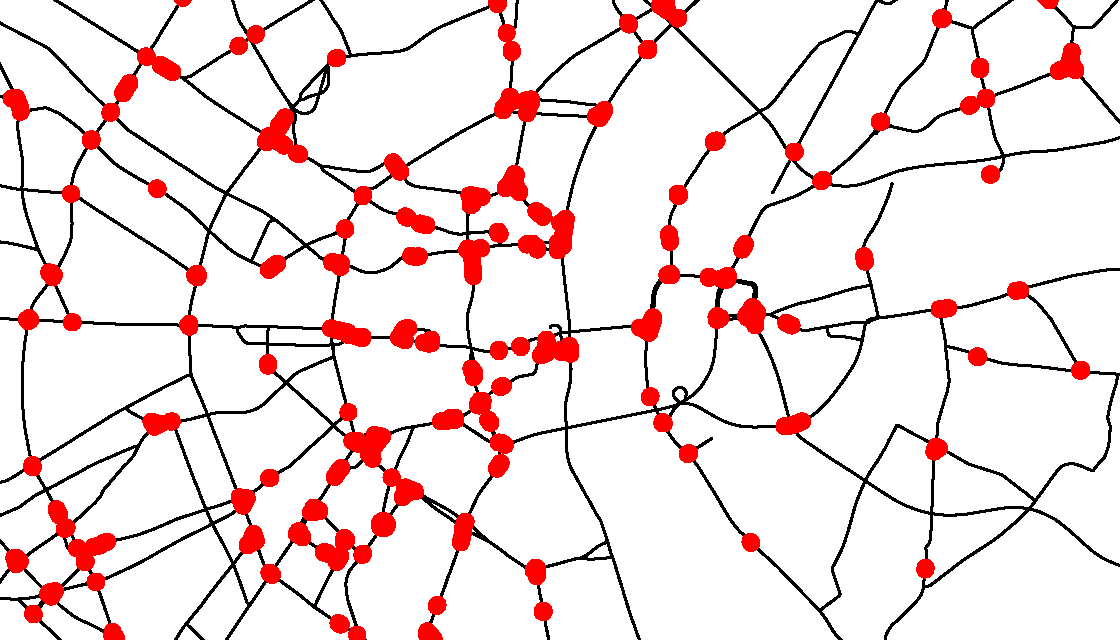
\includegraphics[scale=.9883]{../chapter7/junction-buffer}
	% 1:180000 Google Mercator, bbox 768720 6606550 781320 6613750, 0.2mm stroke
	% true scale at equator => scale at this latitude is approx. 1:113650
	% => scale image down ever so slightly to achieve a "nice" natural scale
	% at a scale of 1:113650, a buffer at 126m distance can be simulated by a stroke width of 1.11mm
	% printf "768720 6610150\n781320 6610150" | cs2cs +init=epsg:3857 +to +proj=merc +lat_ts=50.94 +units=m +datum=WGS84 -
	\caption
		[Pufferung kurzer Linienzüge im Generalisierungsergebnis]
		{Pufferung kurzer Linienzüge (rot) im Generalisierungsergebnis (Köln $\ThousandsScale{115}$)}
	\label{fig:junction-buffer}
}

Einfacher wäre möglicherweise, sich zunutze zu machen, dass der \term{Combiner} die Segmente im Generalisierungsergebnis immer zu möglichst langen Linienzügen verkettet.
Es liegt nahe, dass dort, wo sehr kurze Linienzüge übrig bleiben, wahrscheinlich eine Kreuzung liegt.
Abbildung~\ref{fig:junction-buffer} zeigt beispielhaft einen Puffer mit $\unit[125]{m}$ Distanz von allen Ergebnis"=Linienzügen, deren Länge höchstens $\unit[80]{m}$ beträgt.
Wie zu sehen ist, decken die Puffer tatsächlich viele komplexe Kreuzungen ab.
Eventuell würde es nach der Vereinigung der Pufferflächen bereits genügen, anstelle einer Skelettierung (siehe Abschnitt~\ref{ch:skeleton}) alle Linienzüge, welche den Puffer schneiden, in dessen Schwerpunkt zusammenzuführen.
Zu prüfen wäre jedoch, ob eine verbesserte Auswertung von Attributen (siehe Abschnitt~\ref{ch:improvements-stats}) diesen Ansatz erschwert, indem die Linienzüge häufiger bei Attributwechseln aufgeteilt werden und damit kürzer werden.

Schließlich sei daran erinnert, dass sich \citeauthor{MM99} bereits mit dem Thema der Kreuzungserkennung im Kontext der automatisierten Generalisierung von Straßennetzen auseinandergesetzt haben (siehe Abschnitt~\ref{ch:graph-based}). \cf{MM99}



\subsection{Allgemeine Anwendbarkeit}
% statt nur der gewählte Spezialfall
% vgl. 6.5

Um die Anwendung auf andere Spezialfälle als die in Abschnitt~\ref{ch:case-selection} ausgewählten Richtungsfahrbahnen zu ermöglichen, wäre eine Verallgemeinerung der entwickelten Algorithmen und ihrer Implementierung im \term{Combiner} nötig.

Abschnitt~\ref{ch:result-other-cases} beschreibt zwei konkrete Beispiele für Spezialfälle, auf welche die Ergebnisse dieser Arbeit wahrscheinlich prinzipiell übertragbar sind.
Um Praxistauglichkeit für diese Fälle zu erzielen, müsste der \term{Combiner} es erlauben, die auf den Spezialfall der Richtungsfahrbahnen zugeschnittenen Module zur Laufzeit durch entsprechende andere Module zu ersetzen.
Diese Möglichkeit wurde bei der Implementierung ausdrücklich vorgesehen (Abschnitt~\ref{ch:impl-analyser}), ist jedoch noch nicht voll nutzbar, da dies im Rahmen dieser Arbeit nicht erforderlich war (Abschnitt~\ref{ch:impl-flexibility-efficiency}).
Außerdem wäre eine Lösung zur Kreuzungserkennung erforderlich (Abschnitt~\ref{ch:improvements-junction-detection}), möglicherweise wiederum auf den jeweiligen Spezialfall zugeschnitten.

Es ist jedoch nicht anzunehmen, dass die Anwendung der entwickelten Algorithmen in allen in Abschnitt~\ref{ch:case-comparison} aufgeführten Spezialfällen erfolgreich wäre.
Die Definition für \textproc{Parallel} in Abschnitt~\ref{ch:analyse-algorithm} bringt mit sich, dass gegenüberliegende Segmente nur genau dann analysiert werden, wenn sie sich wenigstens teilweise überlappen.
Bei anthropogenen Parallelen wie gerade den für diese Arbeit zu betrachtenden Richtungsfahrbahnen ist dies normalerweise der Fall.
Segmente von Linienzügen, die natürlich Gewachsenes darstellen, können hingegen -- bei präziser Erfassung, wie sie von \osm\ im Grundsatz angestrebt wird -- derart windschief zueinander liegen, dass eine Überlappung gegenüberliegender Segmente nicht mehr durchgehend gegeben ist.
Eine Übertragung des in dieser Arbeit entwickelten Ansatzes auf solche Spezialfälle wie die in Abschnitt~\ref{vegetation-case-desc} besprochenen Vegetationsgrenzen ist deshalb wahrscheinlich unmöglich.

% Zick-Zack-Problem?



\subsection{Softwarequalität}
\label{ch:improvements-software}

In der Aufgabenstellung war nicht die Entwicklung einer \emph{Softwarelösung,} sondern die Entwicklung von \emph{Algorithmen} gefordert.
Die Implementierung in Software musste erfolgen, um die Praxistauglichkeit der Algorithmen beurteilen zu können (vgl.~\ref{ch:algorithm-overview}), jedoch stand dabei die Qualität der Software selbst nicht im Vordergrund.

In den Abschnitten~\ref{ch:impl-architecture} und~\ref{ch:impl-difficulties} waren bereits Entscheidungen diskutiert worden, die zugunsten einer schnelleren Implementierung qualitative Nachteile mit sich brachten.
Eine Weiterentwicklung der folgenden Aspekte kann die Verwendbarkeit des \term{Combiners} durch den Endnutzer verbessern und wäre deshalb wünschenswert.
%
\begin{itemize}

\item
Die Umwandlung von \osm-Daten in Shapefiles (vgl. Abschnitt~\ref{ch:impl-architecture}) ist zum Teil umständlich.
Es wäre wünschenswert, dass der \term{Combiner} die für \osm\ üblichen Formate XML oder PBF direkt verwenden kann.
% "Osmpbf is a Java/C library to read and write OpenStreetMap PBF files."
Für kleinere Bereiche wäre auch die Möglichkeit einer direkten Abfrage der \osm-Datenbank denkbar.
\cf[233]{RT09}

\item
Die Datenausgabe ist ebenfalls verbesserungsfähig.
Sie sollte in einem Format erfolgen, das die Weiterverwendung innerhalb von \osm\ einfacher macht als die derzeitige Ausgabe als Shapefile.
Das Verketten aller Segmente (vgl. Abschnitt~\ref{ch:impl-generalisation}) sollte womöglich eine optionale Operation sein, da sie nicht für jede denkbare Weiterverarbeitung benötigt wird.
Durch das Verketten ist es zudem schwierig, \term{tags} aus den Eingangsdaten beizubehalten, da sich \term{tags} im Verlauf einer Straße oft ändern.
Deshalb sind bisher nur wenige Attribute überhaupt im Ergebnis enthalten.

\item
Entsprechend Abschnitt~\ref{ch:impl-architecture} wird derzeit als internes Koordinatensystem nur die UTM-Zone~32 verwendet, welche gut zu dem in Kapitel~\ref{ch:result} verwendeten Testdatensatz passt.
% in io.Projection
Um Geodaten aus anderen Regionen der Welt verarbeiten zu können, muss der \term{Combiner} für eine andere UTM-Zone neu kompiliert werden.
Die jeweils am besten passende UTM-Zone ließe sich jedoch auch automatisch anhand der Eingangsdaten ermitteln.
% in io.ShapeReader

\item
% vgl. 6.4 + 5.4.3
In Abschnitt~\ref{ch:impl-flexibility-efficiency} wurde bereits erwähnt, dass die Effizienz des \term{Combiners} Raum für Verbesserungen bietet, insbesondere im Hinblick auf den Speicheraufwand.
Die Laufzeitmessungen in Abschnitt~\ref{ch:result-railways} legen nahe, dass dieser unnötig hoch ist.
Obwohl bereits Änderungen an Parametern dies verbessern können, erscheint eine generelle Verbesserung des Designs sinnvoll.
Beispielsweise könnte die auf Basis von Objekten implementierte Vektor-Mathematik relativ leicht durch statische Methoden ersetzt werden, die ohne zusätzlichen Speicher auskommen.

Auch der Speicheraufwand im Java Collections Framework hat Optimierungspotenzial.
Gegenwärtig werden vom \term{Combiner} zur Implementierung vieler Mengen Datenstrukturen vom Typ \code{LinkedList} genutzt.
Diese bedürfen intern für jedes Element eines zusätzlichen Containerobjekts (\code{LinkedList.Entry}).
Möglicherweise ließe sich der Speicheraufwand durch einen Wechsel auf \code{ArrayList} verringern, geschickt gewählte Anfangskapazitäten vorausgesetzt.

Teile der Algorithmen eignen sich ferner für nebenläufige Ausführung.
Mit entsprechenden Anpassungen könnte die Leistungsfähigkeit moderner Hardware besser ausgenutzt werden.
% https://de.wikipedia.org/wiki/Nebenl%C3%A4ufigkeit

\item
Die Bedienung über die Kommandozeile (CLI) ist zwar ausreichend für das Testen der Algorithmen durch den Entwickler, ist jedoch für den Endnutzer unnötig anspruchsvoll.
\cf[363]{CR03}
Eine graphische Benutzeroberfläche (GUI) würde die Einstiegshürde erheblich senken.
Mit einer Integration in JOSM als \term{plug-in} (Abschnitt~\ref{ch:impl-architecture}) würden sich gleichzeitig die zuvor beschriebenen Probleme beim Einlesen der Ausgangsdaten lösen lassen, da JOSM alle angesprochenen Formate bereits unterstützt.

\end{itemize}

Des Weiteren ist gegenwärtig die Wiederverwendbarkeit des \term{Combiners} und seiner Bestandteile für Entwickler nicht optimal.
Verbesserungen an den folgenden Punkten können sich indirekt auch auf den Endnutzer auswirken, indem sie die Entwicklung von Software mit weniger Fehlern fördern und die Weiterentwicklung vereinfachen.
%
\begin{itemize}

\item
Es besteht gegenwärtig keine nennenswerte Testabdeckung \term{(test coverage).}

\item
Vielerorts wird im \term{Combiner} das objektorientierte Prinzip der Kapselung nicht beachtet, um in Debugging-Ausgaben leichter lesbaren Code zu erzielen.
Während dies in bestimmten Umständen sinnvoll sein kann, ist es für öffentliche Klassen zu vermeiden. \cf[98]{Blo01}
%insb. \texttt{Dataset}  (s. „Big Renaming \#4“)
%evtl. common sink/listener

\item
Wie in Abschnitt~\ref{ch:data-structures-geotools} erwähnt, könnte ein Implementieren der Programmierschnittstelle (\term{application programming interface,} API) für JTS und GeoTools die Verwendung von Bestandteilen des \term{Combiners} in anderen Projekten erleichtern.

\item
Die Dokumentation der API des \term{Combiners} ist noch unvollständig.

\end{itemize}

%2: Dataset
% special uses (to be reconsidered):
% - Output for debugging
% - Corr.Graph to get all segments
% - Gen.Lines to get all segments and to get midPoints
% - AbstractSegment for debugging (parallelFragment sink etc.)
%3: code currently contains a lot of special-cases for debugging as well as testing:
% - pervasive debug output needs to be overhauled; perhaps as a common sink/listener



\subsection{OSM Inspector}
% vgl. insb. 6.2

Der \term{OSM~Inspector} ist ein von der Geofabrik entwickeltes Web-Werkzeug, das Beitragenden helfen kann, bestimmte Fehler in der \osm-Datenbank zu entdecken.
\cf[142]{RT09}
Auch einige Attribute von Linienzügen im \osm-Straßennetz können damit überprüft werden:
„Highways [...] are one of the most important features in OSM.
This [OSM Inspector view] helps finding problems on highways such as missing names, unusal highway types or wrong oneway tags.“
\citex{osm:InspectorHighways}

Bisher kann der \term{OSM~Inspector} für Straßen immer nur einen einzelnen \term{way} prüfen.
Zusammenhänge zwischen mehreren \term{ways}, die Teil derselben Straße sind, können nicht erkannt werden.
Der in Abschnitt~\ref{ch:result-tags} beschriebene Fehler widersprüchlicher Attribute zweier Richtungsfahrbahnen bleibt deshalb im \term{OSM~Inspector} unentdeckt.

Es ist denkbar, dass die Integration einer geometrischen Prüfung auf Parallelität -- wie sie die in dieser Arbeit entwickelten Algorithmen bieten -- in den \term{OSM~Inspector} sinnvoll sein könnte.
Es besteht die Chance, dass viele der angesprochenen Fälle fehlerhafter \term{tags} so durch die \osm-Community beseitigt werden können.
Dies würde die Datenqualität in \osm\ insgesamt erhöhen und damit die automatisierte Weiterverarbeitung nicht nur mit dem \term{Combiner} vereinfachen.

Allerdings ist der \term{Combiner} gegenwärtig nicht auf die Integration in den \term{OSM~Inspector} ausgelegt.
% obige Korrektheit-Probleme, Performance (weltweit?), Java cs. C++ etc.
Es ist auch fraglich, ob die mit einer Integration verbundenen betriebswirtschaftlichen Kosten den potenziellen Nutzen rechtfertigen.
% weitere Tools erwähnen?
% https://wiki.openstreetmap.org/wiki/Quality_assurance#Error_detection_tools



\section{Andere Ansätze und neuere Forschung}
\label{ch:recent-research}

Neben den in Abschnitt~\ref{ch:existing-approaches} besprochenen Ansätzen und der mit dieser Arbeit entwickelten Methode des geometrischen Vergleichs möglichst kurzer Fragmente kommen für das Erkennen und Zusammenfassen paralleler Linienzüge noch weitere Ansätze in Frage.

So wäre denkbar, durch Graphenanalyse Maschen im Straßennetz zu ermitteln und zu prüfen, ob die von ihnen umschlossene Fläche eine solch schmale und lange Form hat, dass es sich um die Fläche zwischen zwei parallelen Linienzügen handeln könnte.

Auch kann der in Abschnitt~\ref{ch:conflict-detection} erwähnte Ansatz von \citeauthor{KP98} nicht mehr grundsätzlich ausgeschlossen werden.
Es ist nicht offensichtlich, dass die mit ihm verbundenen Kosten höher wären als die Kosten der mit der vorliegenden Arbeit entwickelten Methode (siehe Abschnitt~\ref{ch:efficiency}).

Ein neuerer Ansatz wurde von \citeauthor{CTGV14} für Eisenbahnstrecken entwickelt.
Er ähnelt vom Ablauf her der in Abschnitt~\ref{ch:skeleton} beschriebenen Thiessen-Polygon-Methode, jedoch werden die Knoten weniger stark verdichtet und es wird direkt mit dem Ergebnis der Delaunay-Triangulierung weitergearbeitet, anstatt Polygone daraus zu erzeugen.
Der Vergleich zwischen dem entstandenen Dreiecksnetz und den Eingangsdaten ermöglicht es in den meisten Fällen, Gleiskreuzungen und Weichenverbindungen korrekt zu erkennen und zusammenzufassen.
Auf die Möglichkeit der Übertragung dieses Ansatzes auf ein Straßennetz gehen \citeauthor{CTGV14} nicht ein. \cf{CTGV14}

\Citeauthor{Mat17} setzte für den gleichen Problemfall der Bahnachsenermittlung eine neue Funktion%
\footnote{Die Funktion \code{ST\_ApproximateMedialAxis} wurde in PostGIS-Version 2.2.0 hinzugefügt (in 2015).}
% https://postgis.net/docs/manual-2.2/ST_ApproximateMedialAxis.html
% http://postgis.net/2015/10/07/postgis-2.2.0/
in der Geodatenbank PostGIS ein, die anhand eines \term{straight skeleton} ein Polygon auf dessen Mittellinien reduziert (siehe Abschnitt~\ref{ch:skeleton}).
Diese Funktion wendet \citeauthor{Mat17} nur auf Haupt- und Streckengleise an (vgl.~\ref{ch:result-railways}).
Auch sie führt zu Problemen unter anderem im Kreuzungsbereich.
Angesichts der von \citeauthor{Mat17} hierfür gewählten Lösungen erscheint dem Verfasser eine direkte Übertragbarkeit dieses Ansatzes auf den Straßenraum wenig wahrscheinlich. \cf{Mat17}

Nachdem auch diese neueren Ansätze Probleme mit Kreuzungen beschreiben und nur für konkrete Spezialfälle vorgesehen sind, scheint in Anbetracht der Ergebnisse der vorliegenden Arbeit eine automatisierte Kreuzungserkennung
%und -zusammenfassung
ein sinnvoller nächster Schritt zur Lösung der automatisierten Zusammenfassung von Linienzügen zu sein (siehe Abschnitt~\ref{ch:improvements-junction-detection}).
Ob sich der von \citeauthor{CTGV14} für Eisenbahnen hierzu beschriebene Ansatz verallgemeinern ließe, wäre zu prüfen.

Eine offensichtliche Lösung mit allgemeiner Anwendbarkeit für das Problem der Zusammenfassung zeichnet sich derzeit nicht ab.
Mit einer zuverlässigen Kreuzungserkennung wird die eigentliche Zusammenfassung jedoch wahrscheinlich zu einem leicht lösbaren Problem, für das aus verschiedenen Ansätzen derjenige ausgewählt werden kann, der am besten auf den jeweils vorliegenden Problemfall passt.
Im Wesentlichen ginge es dann um Optimierung der Kosten des Verfahrens und um geschickte Ausnutzung der vorhandenen Attribute. \cf[14]{Tho05}



% single-chapter commands
%\onlyinsubfile{\listoffigures}
%\onlyinsubfile{\subfile{../bibliography/Literaturverzeichnis}}
\end{document}
